\documentclass[tikz,border=3pt]{standalone}
\usepackage[T1]{fontenc}
\usepackage{mathptmx}
\usepackage{pgfplots}
\pgfplotsset{compat=1.18}
\pdfinfoomitdate=1
\pdftrailerid{}
\pdfsuppressptexinfo=-1
\pgfplotsset{briefaxis/.style={
font=\fontsize{9}{11}\selectfont, tick label style={text=black},
label style={text=black}, title style={text=black},
axis line style={black,line width=0.6pt}, tick style={black},
axis background/.style={fill=white}, grid style={black!12},
legend style={text=black,font=\fontsize{9}{11}\selectfont,draw=none,fill=white},
unbounded coords=discard}}
\definecolor{briefblue}{HTML}{0072B2}
\definecolor{brieforange}{HTML}{D55E00}
\definecolor{briefgreen}{HTML}{009E73}
\begin{document}
% data_sha256=c378386475a1dfbe87f833ba7f185dd0cd0adde1294499ff2aca8c4de9e2f8f2
\pgfplotsset{briefaxis/.style={
font=\fontsize{9}{11}\selectfont, tick label style={text=black},
label style={text=black}, title style={text=black},
axis line style={black,line width=0.6pt}, tick style={black},
axis background/.style={fill=white}, grid style={black!12},
legend style={text=black,font=\fontsize{9}{11}\selectfont,draw=none,fill=white},
unbounded coords=discard}}
\definecolor{briefblue}{HTML}{0072B2}
\definecolor{brieforange}{HTML}{D55E00}
\definecolor{briefgreen}{HTML}{009E73}

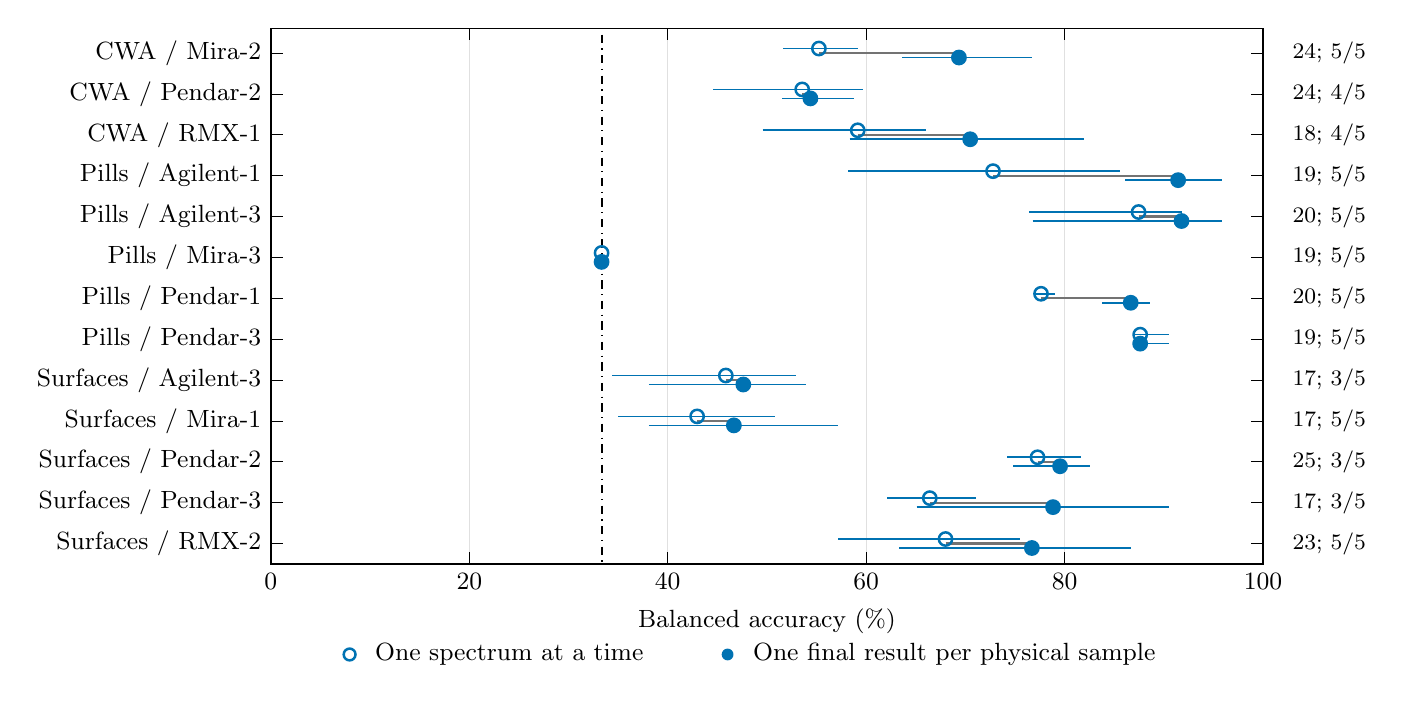
\begin{tikzpicture}
\begin{axis}[briefaxis,width=12.6cm,height=6.8cm,scale only axis,
xmin=0,xmax=100,ymin=-0.6,ymax=12.5,y dir=reverse,
xtick={0,20,40,60,80,100},xmajorgrids=true,
ytick={0,1,2,3,4,5,6,7,8,9,10,11,12},yticklabels={{CWA / Mira-2},{CWA / Pendar-2},{CWA / RMX-1},{Pills / Agilent-1},{Pills / Agilent-3},{Pills / Mira-3},{Pills / Pendar-1},{Pills / Pendar-3},{Surfaces / Agilent-3},{Surfaces / Mira-1},{Surfaces / Pendar-2},{Surfaces / Pendar-3},{Surfaces / RMX-2}},
xlabel={Balanced accuracy (\%)},clip=false]
\draw[black,dash dot,line width=0.7pt] (axis cs:33.333,-0.45) -- (axis cs:33.333,12.5);
\draw[black!55,line width=0.8pt] (axis cs:55.238095238,0) -- (axis cs:69.351851852,0);
\draw[black!55,line width=0.8pt] (axis cs:53.552910053,1) -- (axis cs:54.381613757,1);
\draw[black!55,line width=0.8pt] (axis cs:59.151515151,2) -- (axis cs:70.486111111,2);
\draw[black!55,line width=0.8pt] (axis cs:72.787878788,3) -- (axis cs:91.444444444,3);
\draw[black!55,line width=0.8pt] (axis cs:87.459207459,4) -- (axis cs:91.785714286,4);
\draw[black!55,line width=0.8pt] (axis cs:33.333333333,5) -- (axis cs:33.333333333,5);
\draw[black!55,line width=0.8pt] (axis cs:77.625661376,6) -- (axis cs:86.666666667,6);
\draw[black!55,line width=0.8pt] (axis cs:87.619047619,7) -- (axis cs:87.619047619,7);
\draw[black!55,line width=0.8pt] (axis cs:45.855379189,8) -- (axis cs:47.619047619,8);
\draw[black!55,line width=0.8pt] (axis cs:42.962962963,9) -- (axis cs:46.666666667,9);
\draw[black!55,line width=0.8pt] (axis cs:77.272727273,10) -- (axis cs:79.545454545,10);
\draw[black!55,line width=0.8pt] (axis cs:66.415343915,11) -- (axis cs:78.835978836,11);
\draw[black!55,line width=0.8pt] (axis cs:67.998084291,12) -- (axis cs:76.703703704,12);
\draw[briefblue,line width=0.6pt] (axis cs:51.626984127,-0.11) -- (axis cs:59.206349206,-0.11);
\addplot[only marks,mark=o,mark size=2.4pt,draw=briefblue,fill=white,line width=0.9pt] coordinates {(55.238095238,-0.11)};
\draw[briefblue,line width=0.6pt] (axis cs:44.603174603,0.89) -- (axis cs:59.724867725,0.89);
\addplot[only marks,mark=o,mark size=2.4pt,draw=briefblue,fill=white,line width=0.9pt] coordinates {(53.552910053,0.89)};
\draw[briefblue,line width=0.6pt] (axis cs:49.575757576,1.89) -- (axis cs:66.060606061,1.89);
\addplot[only marks,mark=o,mark size=2.4pt,draw=briefblue,fill=white,line width=0.9pt] coordinates {(59.151515151,1.89)};
\draw[briefblue,line width=0.6pt] (axis cs:58.181818182,2.89) -- (axis cs:85.606060606,2.89);
\addplot[only marks,mark=o,mark size=2.4pt,draw=briefblue,fill=white,line width=0.9pt] coordinates {(72.787878788,2.89)};
\draw[briefblue,line width=0.6pt] (axis cs:76.456876457,3.89) -- (axis cs:91.841491842,3.89);
\addplot[only marks,mark=o,mark size=2.4pt,draw=briefblue,fill=white,line width=0.9pt] coordinates {(87.459207459,3.89)};
\draw[briefblue,line width=0.6pt] (axis cs:33.333333333,4.89) -- (axis cs:33.333333333,4.89);
\addplot[only marks,mark=o,mark size=2.4pt,draw=briefblue,fill=white,line width=0.9pt] coordinates {(33.333333333,4.89)};
\draw[briefblue,line width=0.6pt] (axis cs:76.884920635,5.89) -- (axis cs:79.001322751,5.89);
\addplot[only marks,mark=o,mark size=2.4pt,draw=briefblue,fill=white,line width=0.9pt] coordinates {(77.625661376,5.89)};
\draw[briefblue,line width=0.6pt] (axis cs:86.904761905,6.89) -- (axis cs:90.476190476,6.89);
\addplot[only marks,mark=o,mark size=2.4pt,draw=briefblue,fill=white,line width=0.9pt] coordinates {(87.619047619,6.89)};
\draw[briefblue,line width=0.6pt] (axis cs:34.391534392,7.89) -- (axis cs:52.910052910,7.89);
\addplot[only marks,mark=o,mark size=2.4pt,draw=briefblue,fill=white,line width=0.9pt] coordinates {(45.855379189,7.89)};
\draw[briefblue,line width=0.6pt] (axis cs:35.016835017,8.89) -- (axis cs:50.841750842,8.89);
\addplot[only marks,mark=o,mark size=2.4pt,draw=briefblue,fill=white,line width=0.9pt] coordinates {(42.962962963,8.89)};
\draw[briefblue,line width=0.6pt] (axis cs:74.242424242,9.89) -- (axis cs:81.666666667,9.89);
\addplot[only marks,mark=o,mark size=2.4pt,draw=briefblue,fill=white,line width=0.9pt] coordinates {(77.272727273,9.89)};
\draw[briefblue,line width=0.6pt] (axis cs:62.103174603,10.89) -- (axis cs:71.031746032,10.89);
\addplot[only marks,mark=o,mark size=2.4pt,draw=briefblue,fill=white,line width=0.9pt] coordinates {(66.415343915,10.89)};
\draw[briefblue,line width=0.6pt] (axis cs:57.183908046,11.89) -- (axis cs:75.526819923,11.89);
\addplot[only marks,mark=o,mark size=2.4pt,draw=briefblue,fill=white,line width=0.9pt] coordinates {(67.998084291,11.89)};
\draw[briefblue,line width=0.6pt] (axis cs:63.624338624,0.11) -- (axis cs:76.719576720,0.11);
\addplot[only marks,mark=*,mark size=2.4pt,draw=briefblue,fill=briefblue,line width=0.9pt] coordinates {(69.351851852,0.11)};
\draw[briefblue,line width=0.6pt] (axis cs:51.521164021,1.11) -- (axis cs:58.796296296,1.11);
\addplot[only marks,mark=*,mark size=2.4pt,draw=briefblue,fill=briefblue,line width=0.9pt] coordinates {(54.381613757,1.11)};
\draw[briefblue,line width=0.6pt] (axis cs:58.333333333,2.11) -- (axis cs:81.944444444,2.11);
\addplot[only marks,mark=*,mark size=2.4pt,draw=briefblue,fill=briefblue,line width=0.9pt] coordinates {(70.486111111,2.11)};
\draw[briefblue,line width=0.6pt] (axis cs:86.111111111,3.11) -- (axis cs:95.833333333,3.11);
\addplot[only marks,mark=*,mark size=2.4pt,draw=briefblue,fill=briefblue,line width=0.9pt] coordinates {(91.444444444,3.11)};
\draw[briefblue,line width=0.6pt] (axis cs:76.785714286,4.11) -- (axis cs:95.833333333,4.11);
\addplot[only marks,mark=*,mark size=2.4pt,draw=briefblue,fill=briefblue,line width=0.9pt] coordinates {(91.785714286,4.11)};
\draw[briefblue,line width=0.6pt] (axis cs:33.333333333,5.11) -- (axis cs:33.333333333,5.11);
\addplot[only marks,mark=*,mark size=2.4pt,draw=briefblue,fill=briefblue,line width=0.9pt] coordinates {(33.333333333,5.11)};
\draw[briefblue,line width=0.6pt] (axis cs:83.809523810,6.11) -- (axis cs:88.571428571,6.11);
\addplot[only marks,mark=*,mark size=2.4pt,draw=briefblue,fill=briefblue,line width=0.9pt] coordinates {(86.666666667,6.11)};
\draw[briefblue,line width=0.6pt] (axis cs:86.904761905,7.11) -- (axis cs:90.476190476,7.11);
\addplot[only marks,mark=*,mark size=2.4pt,draw=briefblue,fill=briefblue,line width=0.9pt] coordinates {(87.619047619,7.11)};
\draw[briefblue,line width=0.6pt] (axis cs:38.095238095,8.11) -- (axis cs:53.968253968,8.11);
\addplot[only marks,mark=*,mark size=2.4pt,draw=briefblue,fill=briefblue,line width=0.9pt] coordinates {(47.619047619,8.11)};
\draw[briefblue,line width=0.6pt] (axis cs:38.095238095,9.11) -- (axis cs:57.142857143,9.11);
\addplot[only marks,mark=*,mark size=2.4pt,draw=briefblue,fill=briefblue,line width=0.9pt] coordinates {(46.666666667,9.11)};
\draw[briefblue,line width=0.6pt] (axis cs:74.848484848,10.11) -- (axis cs:82.575757576,10.11);
\addplot[only marks,mark=*,mark size=2.4pt,draw=briefblue,fill=briefblue,line width=0.9pt] coordinates {(79.545454545,10.11)};
\draw[briefblue,line width=0.6pt] (axis cs:65.079365079,11.11) -- (axis cs:90.476190476,11.11);
\addplot[only marks,mark=*,mark size=2.4pt,draw=briefblue,fill=briefblue,line width=0.9pt] coordinates {(78.835978836,11.11)};
\draw[briefblue,line width=0.6pt] (axis cs:63.333333333,12.11) -- (axis cs:86.666666667,12.11);
\addplot[only marks,mark=*,mark size=2.4pt,draw=briefblue,fill=briefblue,line width=0.9pt] coordinates {(76.703703704,12.11)};
\node[anchor=west,text=black,font=\fontsize{8}{10}\selectfont] at (axis cs:102,0) {24; 5/5};
\node[anchor=west,text=black,font=\fontsize{8}{10}\selectfont] at (axis cs:102,1) {24; 4/5};
\node[anchor=west,text=black,font=\fontsize{8}{10}\selectfont] at (axis cs:102,2) {18; 4/5};
\node[anchor=west,text=black,font=\fontsize{8}{10}\selectfont] at (axis cs:102,3) {19; 5/5};
\node[anchor=west,text=black,font=\fontsize{8}{10}\selectfont] at (axis cs:102,4) {20; 5/5};
\node[anchor=west,text=black,font=\fontsize{8}{10}\selectfont] at (axis cs:102,5) {19; 5/5};
\node[anchor=west,text=black,font=\fontsize{8}{10}\selectfont] at (axis cs:102,6) {20; 5/5};
\node[anchor=west,text=black,font=\fontsize{8}{10}\selectfont] at (axis cs:102,7) {19; 5/5};
\node[anchor=west,text=black,font=\fontsize{8}{10}\selectfont] at (axis cs:102,8) {17; 3/5};
\node[anchor=west,text=black,font=\fontsize{8}{10}\selectfont] at (axis cs:102,9) {17; 5/5};
\node[anchor=west,text=black,font=\fontsize{8}{10}\selectfont] at (axis cs:102,10) {25; 3/5};
\node[anchor=west,text=black,font=\fontsize{8}{10}\selectfont] at (axis cs:102,11) {17; 3/5};
\node[anchor=west,text=black,font=\fontsize{8}{10}\selectfont] at (axis cs:102,12) {23; 5/5};
\end{axis}
\draw[briefblue,line width=0.9pt,fill=white] (1, -1.15) circle[radius=0.075];
\node[anchor=west,text=black,font=\fontsize{9}{11}\selectfont] at (1.2,-1.15) {One spectrum at a time};
\fill[briefblue] (5.8,-1.15) circle[radius=0.075];
\node[anchor=west,text=black,font=\fontsize{9}{11}\selectfont] at (6,-1.15) {One final result per physical sample};
\end{tikzpicture}\end{document}
